\documentclass[a0paper,landscape,final]{baposter}

\usepackage{times}
\usepackage{calc}
\usepackage{graphicx}
\usepackage{amsmath}
\usepackage{amssymb}
\usepackage{relsize}
\usepackage{multirow}
\usepackage{bm}
\usepackage{algorithm}
\usepackage{algorithmic}
\usepackage{subfigure}
\usepackage{slashbox}

\usepackage{graphicx}
\usepackage{multicol}

\usepackage{pgfbaselayers}
\pgfdeclarelayer{background}
\pgfdeclarelayer{foreground}
\pgfsetlayers{background,main,foreground}

\usepackage{helvet}
%\usepackage{bookman}
\usepackage{palatino}

\usepackage{enumitem}


\newcommand{\captionfont}{\footnotesize}

%\selectcolormodel{cmyk}

\graphicspath{{fig/}}

%%%%%%%%%%%%%%%%%%%%%%%%%%%%%%%%%%%%%%%%%%%%%%%%%%%%%%%%%%%%%%%%%%%%%%%%%%%%%%%%
%%%% Some math symbols used in the text
%%%%%%%%%%%%%%%%%%%%%%%%%%%%%%%%%%%%%%%%%%%%%%%%%%%%%%%%%%%%%%%%%%%%%%%%%%%%%%%%
% Format
\newcommand{\Matrix}[1]{\begin{bmatrix} #1 \end{bmatrix}}
\newcommand{\Vector}[1]{\Matrix{#1}}
\newcommand*{\SET}[1]  {\ensuremath{\mathcal{#1}}}
\newcommand*{\MAT}[1]  {\ensuremath{\mathbf{#1}}}
\newcommand*{\VEC}[1]  {\ensuremath{\bm{#1}}}
\newcommand*{\CONST}[1]{\ensuremath{\mathit{#1}}}
\newcommand*{\norm}[1]{\mathopen\| #1 \mathclose\|}% use instead of $\|x\|$
\newcommand*{\abs}[1]{\mathopen| #1 \mathclose|}% use instead of $\|x\|$
\newcommand*{\absLR}[1]{\left| #1 \right|}% use instead of $\|x\|$

\def\norm#1{\mathopen\| #1 \mathclose\|}% use instead of $\|x\|$
\newcommand{\normLR}[1]{\left\| #1 \right\|}% use instead of $\|x\|$

%%%%%%%%%%%%%%%%%%%%%%%%%%%%%%%%%%%%%%%%%%%%%%%%%%%%%%%%%%%%%%%%%%%%%%%%%%%%%%%%
% Multicol Settings
%%%%%%%%%%%%%%%%%%%%%%%%%%%%%%%%%%%%%%%%%%%%%%%%%%%%%%%%%%%%%%%%%%%%%%%%%%%%%%%%
\setlength{\columnsep}{0.7em}
\setlength{\columnseprule}{0mm}


%%%%%%%%%%%%%%%%%%%%%%%%%%%%%%%%%%%%%%%%%%%%%%%%%%%%%%%%%%%%%%%%%%%%%%%%%%%%%%%%
% Save space in lists. Use this after the opening of the list
%%%%%%%%%%%%%%%%%%%%%%%%%%%%%%%%%%%%%%%%%%%%%%%%%%%%%%%%%%%%%%%%%%%%%%%%%%%%%%%%
\newcommand{\compresslist}{%
\setlength{\itemsep}{1pt}%
\setlength{\parskip}{0pt}%
\setlength{\parsep}{0pt}%
}


%%%%%%%%%%%%%%%%%%%%%%%%%%%%%%%%%%%%%%%%%%%%%%%%%%%%%%%%%%%%%%%%%%%%%%%%%%%%%%
%%% Begin of Document
%%%%%%%%%%%%%%%%%%%%%%%%%%%%%%%%%%%%%%%%%%%%%%%%%%%%%%%%%%%%%%%%%%%%%%%%%%%%%%

\begin{document}

%%%%%%%%%%%%%%%%%%%%%%%%%%%%%%%%%%%%%%%%%%%%%%%%%%%%%%%%%%%%%%%%%%%%%%%%%%%%%%
%%% Here starts the poster
%%%---------------------------------------------------------------------------
%%% Format it to your taste with the options
%%%%%%%%%%%%%%%%%%%%%%%%%%%%%%%%%%%%%%%%%%%%%%%%%%%%%%%%%%%%%%%%%%%%%%%%%%%%%%
\typeout{Poster Starts}
\background{
  \begin{tikzpicture}[remember picture,overlay]%
   \draw (current page.north west)+(-2em,-0em) node[anchor=north west] {\hspace{-2em}\includegraphics[height=1.1\textheight]{silhouettes_background}};
 \end{tikzpicture}%
}
\definecolor{blue}{RGB}{150,200,242}
\definecolor{darkblue}{RGB}{68,92,170}
\definecolor{brown}{RGB}{245,236,215}

\begin{poster}{
  % Show grid to help with alignment
  grid=false,
  % Column spacing
  colspacing=1em,
  % Color style
  %headerColorOne=cyan!20!white!90!black,
  %borderColor=cyan!30!white!90!black,
  %bgColorOne=cyan!10!white,
  headerColorOne=blue,
  borderColor=darkblue,
  bgColorOne=brown,
  boxColorOne=white,
  %bgColorOne=lighteryellow,
  %bgColorTwo=lightestyellow,
  %borderColor=reddishyellow,
  %headerColorOne=yellow,
  %headerColorTwo=reddishyellow,
  %headerFontColor=black,
  %boxColorOne=lightyellow,
  %boxColorTwo=lighteryellow,
  % Format of textbox
  textborder=roundedleft,
  % Format of text header
  eyecatcher=true,
  headerborder=open,
  headerheight=0.08\textheight,
  headershape=roundedright,
  headershade=plain,
  headerfont=\Large\textsf, %Sans Serif
  boxshade=plain,
%  background=shade-tb,
  background=plain,
  linewidth=2pt,
  columns=3
  }
  % Eye Catcher
  {{\begin{minipage}{1.5cm}
    \vspace{0.5cm}
	
\includegraphics[width=5cm]{ethzlogo}
\end{minipage}}
  } % No eye catcher for this poster. If an eye catcher is present, the title is centered between eye-catcher and logo.
  % Title
  {\sf %Sans Serif
  %\bf% Serif
  {\huge Online Learning with Expert Advice for Sports Betting}}
  % Authors
  {\sf %Sans Serif
  % Serif
  Matteo Turchetta\hspace{1cm}
  Riccardo Moriconi\hspace{1cm}
  Yijun Pan\\
  }
%  {{\begin{minipage}{1.5cm}	
\includegraphics[width=2.5cm]{fig/usclogo.pdf}
%    \end{minipage}}
%  }
  % University logo
  
  \tikzstyle{light shaded}=[top color=baposterBGtwo!30!white,bottom color=baposterBGone!30!white,shading=axis,shading angle=30]

  % Width of left inset image
     \newlength{\leftimgwidth}
     \setlength{\leftimgwidth}{0.78em+8.0em}

%%%%%%%%%%%%%%%%%%%%%%%%%%%%%%%%%%%%%%%%%%%%%%%%%%%%%%%%%%%%%%%%%%%%%%%%%%%%%%
%%% Now define the boxes that make up the poster
%%%---------------------------------------------------------------------------
%%% Each box has a name and can be placed absolutely or relatively.
%%% The only inconvenience is that you can only specify a relative position
%%% towards an already declared box. So if you have a box attached to the
%%% bottom, one to the top and a third one which should be in between, you
%%% have to specify the top and bottom boxes before you specify the middle
%%% box.
%%%%%%%%%%%%%%%%%%%%%%%%%%%%%%%%%%%%%%%%%%%%%%%%%%%%%%%%%%%%%%%%%%%%%%%%%%%%%%
    %
    % A coloured circle useful as a bullet with an adjustably strong filling
    \newcommand{\colouredcircle}[1]{%
      \tikz{\useasboundingbox (-0.2em,-0.32em) rectangle(0.2em,0.32em); \draw[draw=black,fill=baposterBGone!80!black!#1!white,line width=0.03em] (0,0) circle(0.18em);}}

%%%%%%%%%%%%%%%%%%%%%%%%%%%%%%%%%%%%%%%%%%%%%%%%%%%%%%%%%%%%%%%%%%%%%%%%%%%%%%
  \headerbox{Overview}{name=overview,column=0,row=0}{
%%%%%%%%%%%%%%%%%%%%%%%%%%%%%%%%%%%%%%%%%%%%%%%%%%%%%%%%%%%%%%%%%%%%%%%%%%%%%%
{\bf Goal}

Apply online learning algorithms to derive profitable sport bets without prior knowledge of the games.

\vspace{0.07cm}
{\bf Online Learning with Expert Advice}
\vspace{-0.2cm}
\begin{itemize}[leftmargin=*]\compresslist
    %\setlength{\itemindent}{-1em}
	\item[-] The learner is given a pool of experts ({\bf bookmakers}) which provide advices in the form of forecasts ({\bf odds}) over the outcome of an event ({\bf sport game}). 
	\item[-] Experts are assigned weights based on their credits. 
	\item[-] The concept of credibility is defined on the loss function.
\end{itemize}
  
  
  }

%%%%%%%%%%%%%%%%%%%%%%%%%%%%%%%%%%%%%%%%%%%%%%%%%%%%%%%%%%%%%%%%%%%%%%%%%%%%%%
  \headerbox{Learning Algorithm}{name=algorithm, column=0,below=overview}{
%%%%%%%%%%%%%%%%%%%%%%%%%%%%%%%%%%%%%%%%%%%%%%%%%%%%%%%%%%%%%%%%%%%%%%%%%%%%%%
 \vspace{-0.4cm}
\begin{algorithm}[H]
\caption{Weighted Average Algorithm}
\begin{algorithmic}[1]
 \STATE ${w_0^k} = 1/K, k = 1,...,K$
\FORALL {$t = 1:N$}
    \STATE Experts announce predictions $\gamma _t^k \in \Gamma ,k = 1,...,K$
    \STATE Algorithm announces ${\gamma _t} = \frac{{\sum {w_t^k\gamma _t^k} }}{{\sum {w_t^k} }}$
    \STATE Reality announces ${\omega _t} \in \Omega$
    \STATE $w_t^k = w_{t - 1}^k{e^{ - \eta \lambda ({\omega _N},\lambda _t^k)}}$
\ENDFOR
\end{algorithmic}
\label{alg:inf}
\end{algorithm}
\vspace{-0.7cm}
\begin{itemize}[leftmargin = *]\compresslist
    \item[-] Similarly, for Follow the Leader Algorithm, predication function is maximisation instead of weighted mean.
\end{itemize}
\vspace{-0.3cm}
\begin{algorithm}[H]
\caption{Strong Aggregating Algorithm}
\begin{algorithmic}[1]
 \STATE ${w_0^k} = 1/K, k = 1,...,K$
\FORALL {$t = 1:N$}
    \STATE Experts announce predictions $\gamma _t^k \in \Gamma ,k = 1,...,K$
    \STATE Generalised predication ${g_t}(\omega ) =  - \frac{1}{\eta }\ln \sum\limits_{k = 1}^K {{w_k}} {e^{ - \eta \lambda (\omega ,\gamma _t^k)}},\forall \omega  \in \Omega$
    \STATE Algorithm announces ${\gamma _t} = S({g_t}) \in \Gamma$
    \STATE Reality announces ${\omega _t} \in \Omega$
    \STATE $w_t^k = w_{t - 1}^k{e^{ - \eta \lambda ({\omega _N},\lambda _t^k)}}$
\ENDFOR
\end{algorithmic}
\label{alg:inf}
\end{algorithm}
\vspace{-0.7cm}
\begin{itemize}[leftmargin = *]\compresslist
    \item[-] For Brier Loss ($l2$ squared norm), the substitution function $S$ is ${\gamma _k}\{ \omega \}  = {\rm{ }}{(s - {g_k}(\omega ))^ + }/2$, where ${\sum\nolimits_{\omega  \in \Omega } {(s - {g_k}(\omega ))} ^ + } = 2$.
\end{itemize}
\vspace{-0.3cm}

  }
  
    %%%%%%%%%%%%%%%%%%%%%%%%%%%%%%%%%%%%%%%%%%%%%%%%%%%%%%%%%%%%%%%%%%%%%%%%%%%%%%
  \headerbox{Probability Extraction}{name=prob, column=0, below=algorithm, above=bottom}{
%%%%%%%%%%%%%%%%%%%%%%%%%%%%%%%%%%%%%%%%%%%%%%%%%%%%%%%%%%%%%%%%%%%%%%%%%%%%%%
We use [Vovk09] to extract probability estimation from odds. Given the odds ($o_h, o_d, o_a$), solve $\gamma$ such that:
\[\frac{1}{{{o_h^\gamma }}} + \frac{1}{{{o_d^\gamma }}} + \frac{1}{{{o_a^\gamma }}} = 1\]
Then we have $P_h = o_h^{-\gamma}$, $P_d = o_d^{-\gamma}$, $P_a = o_a^{-\gamma}$.

  }
  
  
    %%%%%%%%%%%%%%%%%%%%%%%%%%%%%%%%%%%%%%%%%%%%%%%%%%%%%%%%%%%%%%%%%%%%%%%%%%%%%%
  \headerbox{Loss Function}{name=loss, column=1}{
%%%%%%%%%%%%%%%%%%%%%%%%%%%%%%%%%%%%%%%%%%%%%%%%%%%%%%%%%%%%%%%%%%%%%%%%%%%%%%
The proposed loss functions are minimised when the predicted distribution coincides with the true probability distribution ( {\bf Proper Scoring Rule}).

\vspace{0.2cm}
{\bf Brier Loss}

In this case the target distribution ${\delta _\omega}$ is a Dirac distribution concentrated at the actual outcome y of the match.

\[\ell \left( {\gamma ,\underline \omega  } \right) = \sum\limits_{\omega  \in \Omega } {{{\left( {\gamma \left( \omega  \right) - {\delta _{\underline \omega  }}\left( \omega  \right)} \right)}^2}} \]
{\bf Calibration Loss}

A forecaster is $\epsilon$-calibrated if:
\[P\left( {\omega  = \omega_*|\gamma \left( \omega_* \right) \in \left[ {p - \varepsilon ;p + \varepsilon } \right]} \right) \approx p,\varepsilon  > 0\]

In practise, reality does not reveal the true probability distribution. But we can approximate through relative frequency $ $ and use it as target distribution. 
Thus the calibration loss function can be defined as
\[\ell \left( \gamma  \right) = \sum\limits_{\omega  \in \Omega } {{{\left( {{{\hat P}_\omega } - \gamma \left( \omega  \right)} \right)}^2}} \]
Multiple loss functions can be derived by replacing the $l2$ norm.
\vspace{-0.2cm}
\begin{itemize}[leftmargin = *]\compresslist
    \item[-] KL divergence (logarithmic loss)
    \item[-] $l1$ norm
\end{itemize}
\vspace{-0.3cm}

  }
  
%%%%%%%%%%%%%%%%%%%%%%%%%%%%%%%%%%%%%%%%%%%%%%%%%%%%%%%%%%%%%%%%%%%%%%%%%%%%%%
  \headerbox{Results}{name=results,column=1, below=loss, above=bottom}{
%%%%%%%%%%%%%%%%%%%%%%%%%%%%%%%%%%%%%%%%%%%%%%%%%%%%%%%%%%%%%%%%%%%%%%%%%%%%%%
{\bf Dataset}
\vspace{-0.2cm}
\begin{itemize}[leftmargin=*]\compresslist
    \item[-] A total of 11624 games from 6 different leagues over 7 years.
    \item[-] 10 bookmakers with odds ($1X2$) for every game.
    \item[-] Use 2170 games from 1 league (England Premier League) as training data. The rest 9454 games are testing data.
\end{itemize}

{\bf Regret}

 The following plots show the regret (in the form of difference between cumulative loss of the algorithm and that of every bookmaker) of the Weighted Average Algorithm with Brier loss and $\epsilon$-Calibration loss.
 
 \vspace{-0.2cm}
\begin{itemize}[leftmargin=*]\compresslist
    \item[-]  {\bf $l1$ norm}
\end{itemize}
\vspace{-0.5cm}
 
 \begin{figure}[H]
    \centering
    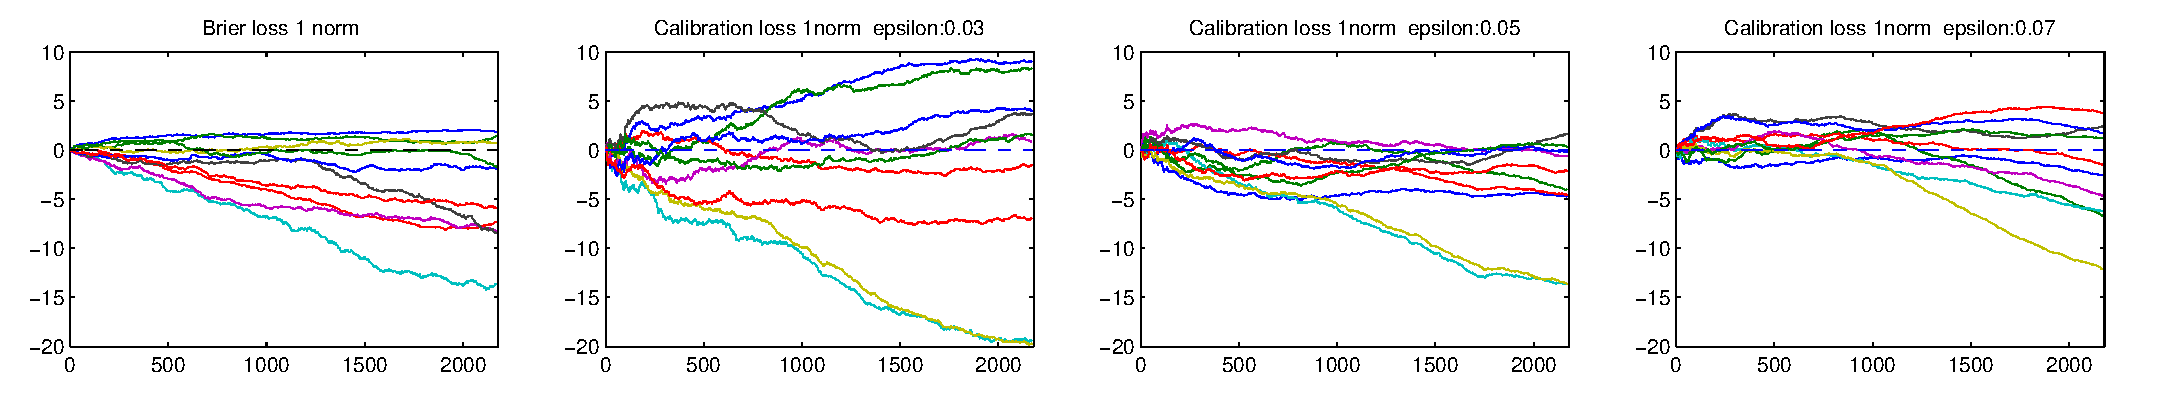
\includegraphics[width = \linewidth]{fig/exp/1norm.eps}
\end{figure}
 
 \vspace{-0.8cm}
\begin{itemize}[leftmargin=*]\compresslist
    \item[-]  {\bf $l2$ norm}
\end{itemize}
\vspace{-0.5cm}

 \begin{figure}[H]
    \centering
    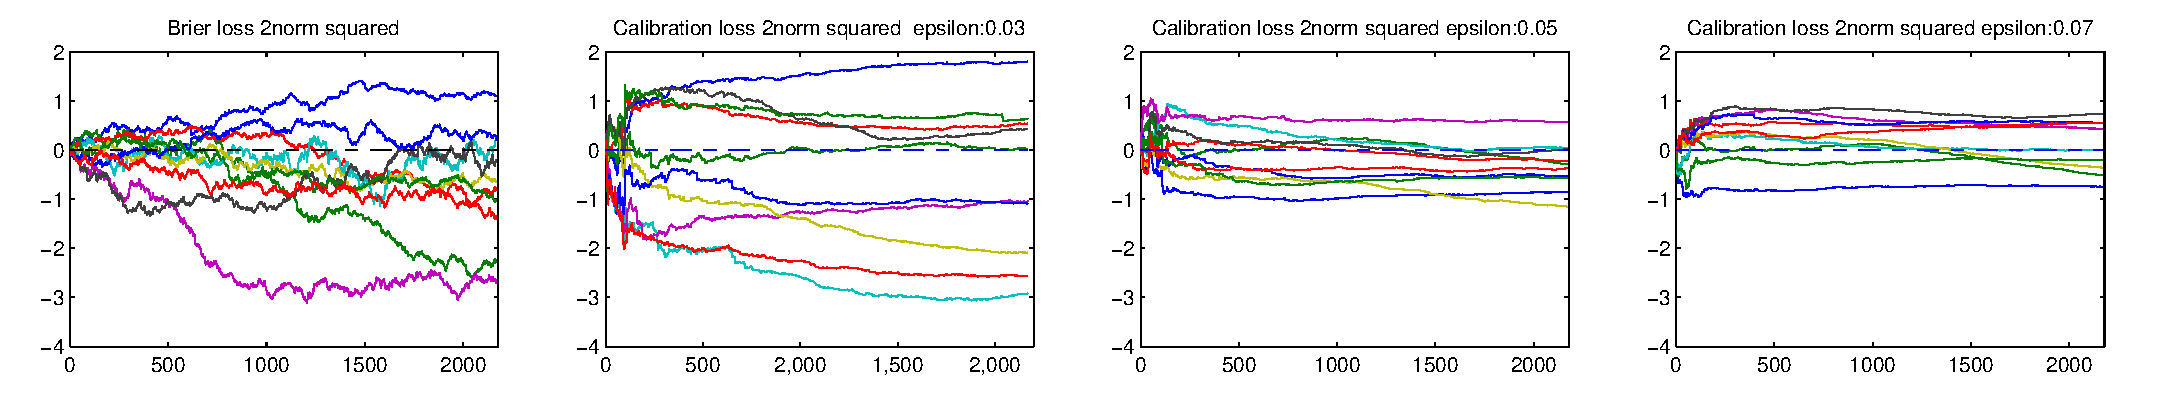
\includegraphics[width = \linewidth]{fig/exp/2norm.eps}
\end{figure}

}


%%%%%%%%%%%%%%%%%%%%%%%%%%%%%%%%%%%%%%%%%%%%%%%%%%%%%%%%%%%%%%%%%%%%%%%%%%%%%%
  \headerbox{Results}{name=resultscon,column=2}{
%%%%%%%%%%%%%%%%%%%%%%%%%%%%%%%%%%%%%%%%%%%%%%%%%%%%%%%%%%%%%%%%%%%%%%%%%%%%%%
  
{\bf Betting Strategy}

\vspace{-0.2cm}
\begin{itemize}[leftmargin=*]\compresslist
    \item[-] Two criteria (probability threshold \& maximum probability expectation threshold) for the betting strategies are effective.
\end{itemize}
\vspace{-0.5cm}

 \begin{figure}[H]
    \centering
    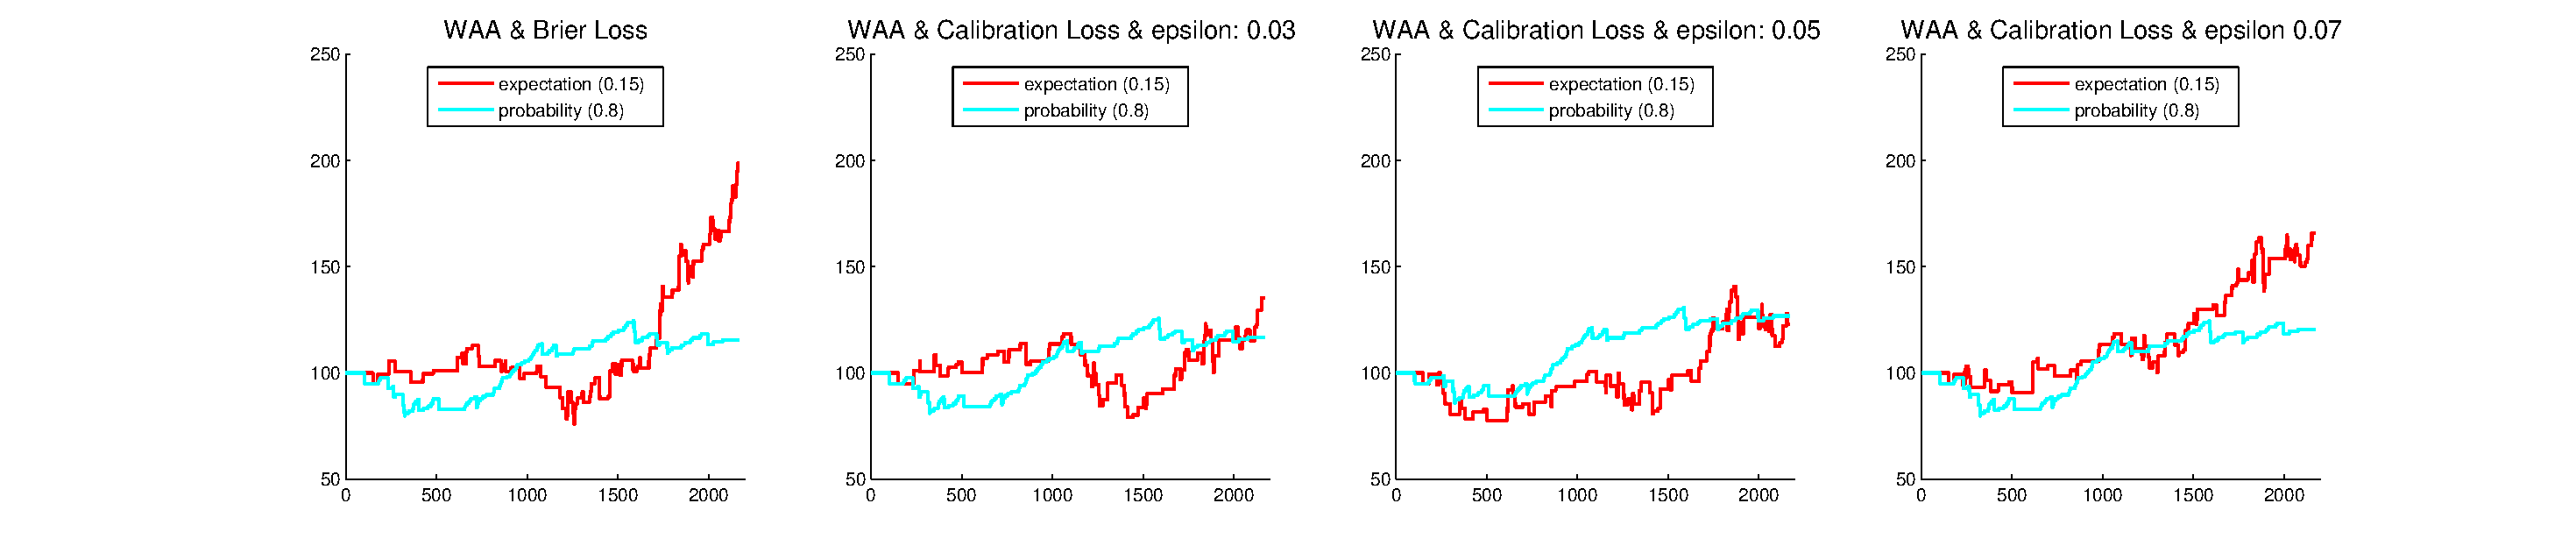
\includegraphics[width = \linewidth]{fig/exp/ep_compare.eps}
\end{figure}

\vspace{-0.5cm}
\begin{itemize}[leftmargin=*]\compresslist
    \item[-] Depending solely on the margin expectation leads to poor performance.  
    \end{itemize}
\vspace{-0.5cm}

\begin{figure}[H]
    \centering
    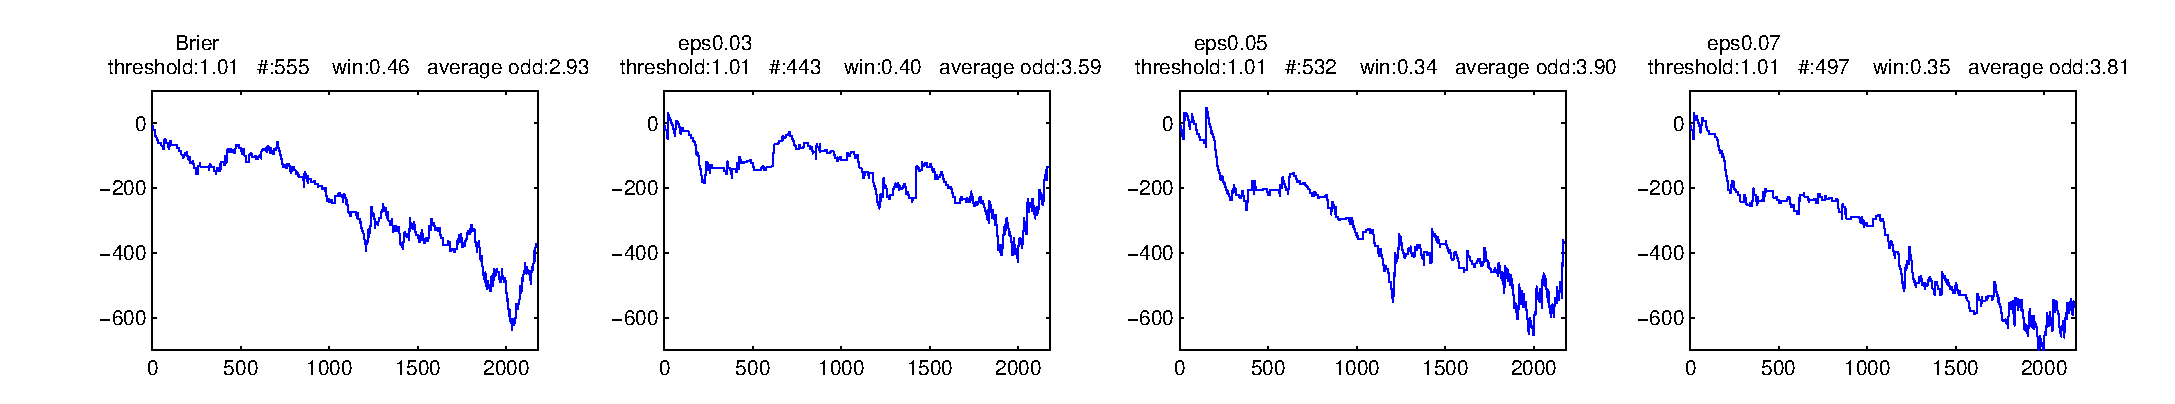
\includegraphics[width = \linewidth]{fig/exp/exponly.eps}
\end{figure}

{\bf Betting Simulation}
\vspace{-0.2cm}
\begin{itemize}[leftmargin=*]\compresslist
    \item[-] Simulation on the testing data.
    \item[-] 100 rounds as burn-in time.
    \item[-] Baseline \textit{Follow the Leader}: follow the bookmaker with highest weights.    
        \item[-] Baseline \textit{Best Bookmaker}: best performance of 10 bookmakers based on overall profit.
\end{itemize}
\vspace{-0.7cm}
 
  \begin{figure}[H]
    \centering
    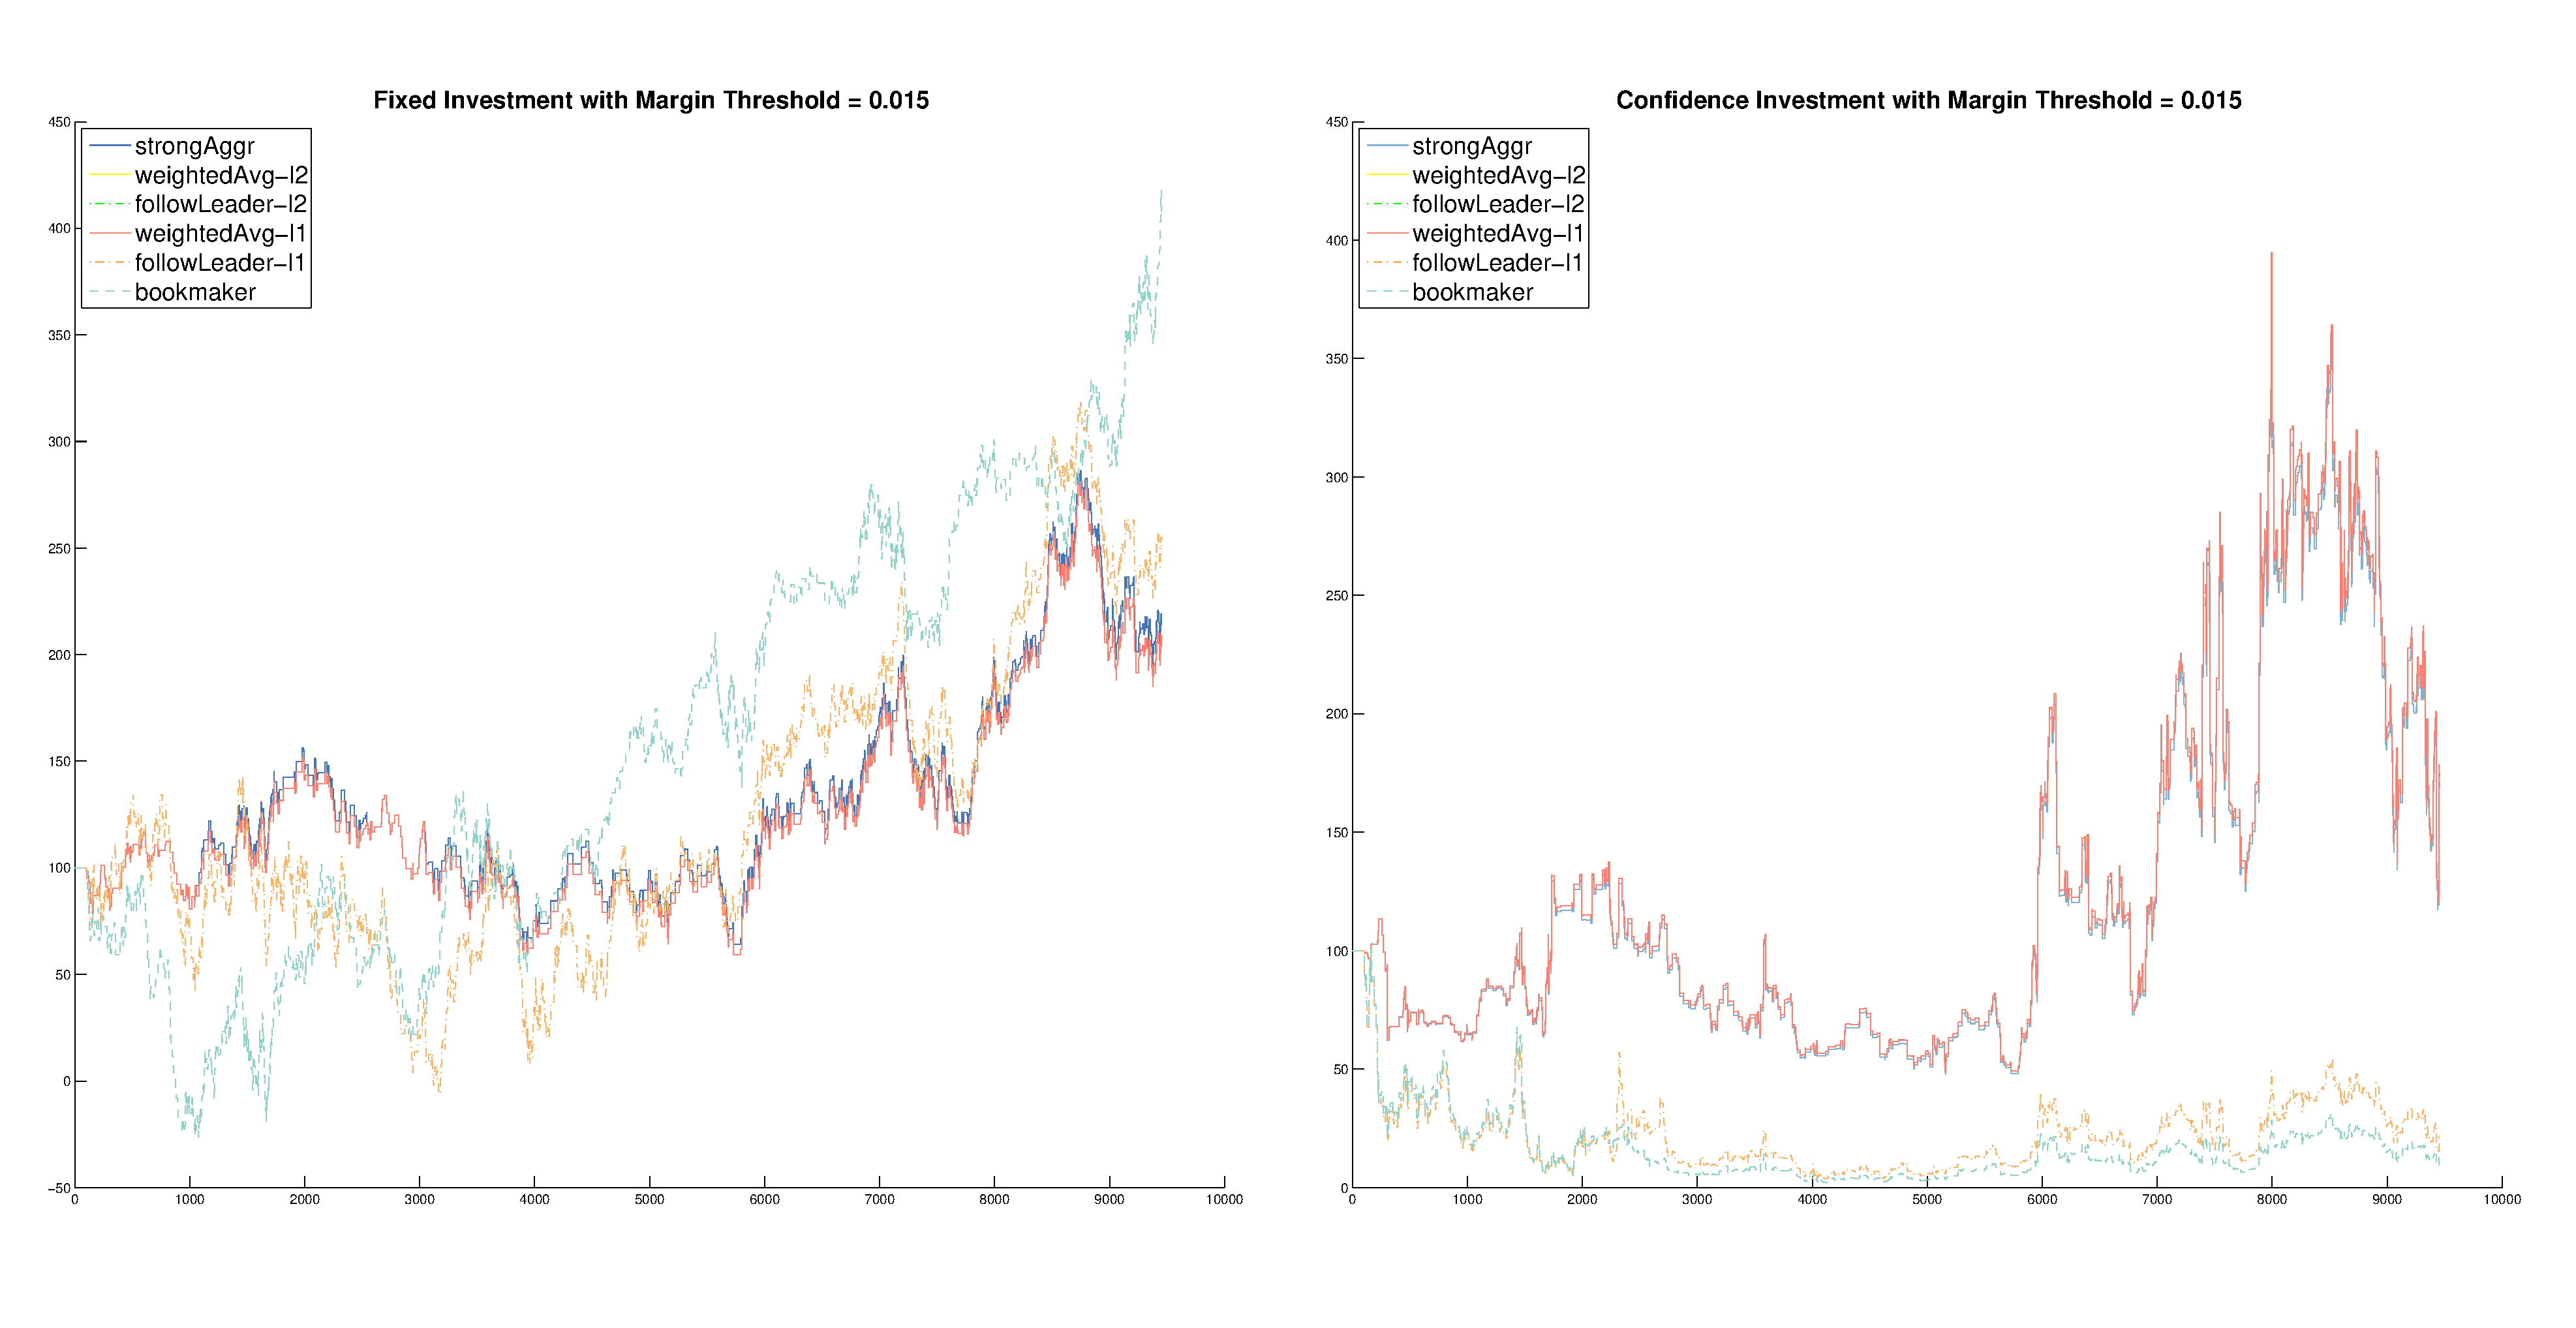
\includegraphics[width = \linewidth]{fig/exp/expectation_both.eps}
\end{figure}
 
 
  }


%%%%%%%%%%%%%%%%%%%%%%%%%%%%%%%%%%%%%%%%%%%%%%%%%%%%%%%%%%%%%%%%%%%%%%%%%%%%%%
  \headerbox{Conclusion}{name=conclusion,column=2,below=resultscon, above = bottom}{
%%%%%%%%%%%%%%%%%%%%%%%%%%%%%%%%%%%%%%%%%%%%%%%%%%%%%%%%%%%%%%%%%%%%%%%%%%%%%%
  \begin{itemize}[leftmargin=*]\compresslist
    \item[-] Bookmakers provide biased probability estimation.
    \item[-] A profitable margin exists for carefully designed betting strategies even without the integration of event features. Although it is very small compared with bookmakers' own profit estimation.
    \item[-] Measurement based solely on calibration without resolution for probability forecasting can be misleading.    
\end{itemize}
  }


\end{poster}%
%
\end{document}
